\begin{frame}{Outline}
    \tableofcontents
\end{frame}

\section{问题定义}
\begin{frame}{问题定义}
    \centering
    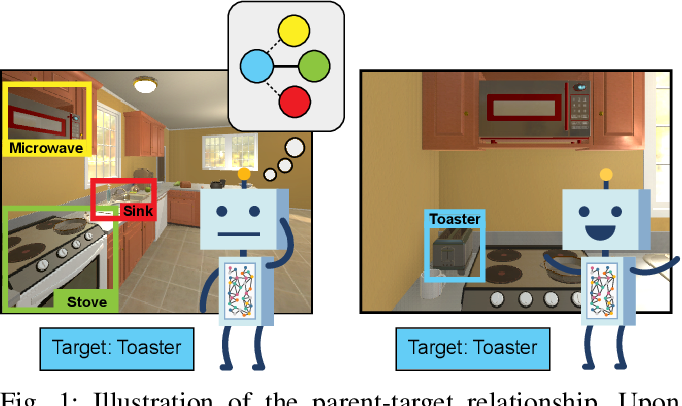
\includegraphics[width=11cm,trim=0 20 0 0,clip]{assets/problem.png}
    \note{
        假设一个agent在一个陌生的环境里,它的目标是要找到一个给定的类别的物体实例。它一开始在环境中的一个随机位置,要求根据感官信息不断移动,最终找到目标物体。
    }
\end{frame}

%\subsection{常见规约和方法}

%\subsection{创新点}

\section{方案总览}
\begin{frame}{方案总览}
    \begin{itemize}
        \item 感知部分
        \item 决策部分
    \end{itemize}
\end{frame}

\section{任务分配}
\begin{frame}{任务分配}
    \begin{table}[h]
        \centering
        \begin{tabular}{cc}
            \toprule
            任务 & 负责人\\
            \midrule
            感知部分 & 彭泽,王子鉴\\
            决策部分 & 姚梦雨,马文洁\\
            \bottomrule
        \end{tabular}
    \end{table}
\end{frame}